\documentclass[]{article}
\usepackage[spanish]{babel}
\usepackage{amsmath, amssymb}
\usepackage{lipsum}
\usepackage{graphicx}
\usepackage{xcolor}

% Agreguemos el paquete array
\usepackage{array}

\title{CDE LATEX }
\author{Clase 5}
\date{27 de marzo del 2023}

\begin{document}

\maketitle

\begin{abstract}
	\lipsum[2]
\end{abstract}

\section{El entorno tabular}
\noindent Sintaxis

\begin{verbatim}
\begin{tabular}[posicion]{Definicion}
a_{11} & a_{12} & a_{13} \\
a_{21} & a_{22} & a_{23}
\end{tabular}
\end{verbatim}

Profundicemos en el argumento \verb*|Definicion|:
Definiremos el numero de columnas y la justificación
de cada una de esas columnas.
\begin{itemize}
\item Usar las letras \verb*|l| (left), \verb*|c| (center) y \verb*|r| (right) para justificar el 
texto dentro de cada columna
\begin{verbatim}
\begin{tabular}[]{lrrc}
	a_{11} & a_{12} & a_{13} & a_{14} \\
	a_{21} & a_{22} & a_{23} & a_{24}
\end{tabular}
\end{verbatim}

Veamos un ejemplo :

\begin{tabular}[]{lrrc}
	$a_{11}$ & $a_{12}$ & $a_{13}$ & $a_{14}$ \\
	$a_{21}$ & $a_{22}$ & $a_{23}$ & $a_{24}$
\end{tabular}

Veamos otro ejemplo :

\begin{tabular}[]{lrrc}
	$a_{11}$ & $a_{12}$ & $a_{13}$ & $a_{14}$ \\
	$a_{21}$ & $a_{22}$ & $a_{23}$ & \lipsum[2]
\end{tabular}

\item Definamos un párrafo como elemento de un 
\verb*|tabular|

Veamos un ejemplo :

\begin{tabular}[]{lrrp{9cm}}
	$a_{11}$ & $a_{12}$ & $a_{13}$ & $a_{14}$ \\
	$a_{21}$ & $a_{22}$ & $a_{23}$ & \lipsum[2]
\end{tabular}
\end{itemize}


\section{Agreguemos lineas horizontales y verticales a tabular}


\noindent Sintaxis

\begin{verbatim}
	\begin{tabular}[posicion]{Definicion}
		a_{11} & a_{12} & a_{13} \\
		a_{21} & a_{22} & a_{23}
	\end{tabular}
\end{verbatim}

Notar el uso de \verb*|hline| y la barra vertical 


\begin{verbatim}
	\begin{tabular}[]{|c|c|c|}
		\hline
		a_{11} & a_{12} & a_{13} \\
		\hline \\
		\hline
		a_{21} & a_{22} & a_{23}
		\hline
	\end{tabular}
\end{verbatim}

En ejecución :

\begin{center}
	\begin{tabular}[]{|c|c|c|}
	\hline
	$a_{11}$ & $a_{12}$ & $a_{13}$ \\
	\hline
	$a_{21}$ & $a_{22}$ & $a_{23}$\\
	\hline
	$a_{21}$ & $a_{22}$ & $a_{23}$\\
	\hline
	$a_{21}$ & $a_{22}$ & $a_{23}$\\
	\hline
	$a_{21}$ & $a_{22}$ & $a_{23}$\\
	\hline
	$a_{21}$ & $a_{22}$ & $a_{23}$\\
	\hline
	$a_{21}$ & $a_{22}$ & $a_{23}$\\
	\hline	
\end{tabular}
\end{center}



\subsection{cline}
El comando \verb*|cline{i-j}| trazara la linea 
horizontal entre la columnas de la \verb*|i|
a la \verb*|j|.
\begin{center}
\begin{tabular}{cccr}
\hline
Producto & Precio Unitario & Cantidad & Subtotal \\
\hline
Monitores & 1250 & 2 & 2500\\
		  & 2780 & 2 & 5560 \\
		  & 16800 & 4 & 67200 \\
\hline
GPU	 	  & 2500 & 2 & 5000\\
          & 3700 & 3 & 11100\\
          \cline{4-4}
          &      &   & 78300

\end{tabular}
\end{center}

\subsection{Encolumnar el punto decimal}
Consideremos que tenemos 4 números punto flotante
, donde cada uno de estos números posee una distinta
cantidad de cifras en la mantisa : 3.14159 , 2.71,
123.4567 y 0.

\begin{center}
\begin{tabular}{cl}
	\hline
	Var1 & 3.14159\\
	Var2 & 2.71\\
	Var3 & 123.4567\\
	Var4 & 0\\
	\hline
\end{tabular}
\end{center}

Consideremos arreglar/encolumnar la ubicación del punto decimal .

\begin{center}
	\begin{tabular}{cr@{.}l}
		Var & NUmeritos & \\
		\hline
		Var1 & 3&14159\\
		Var2 & 2&71\\
		Var3 & 123&4567\\
		Var4 & 0&\\
		\hline
	\end{tabular}
\end{center}

\section{Construcción del indice de figuras}
\lipsum[2-5]

\begin{figure}[h]
\centering
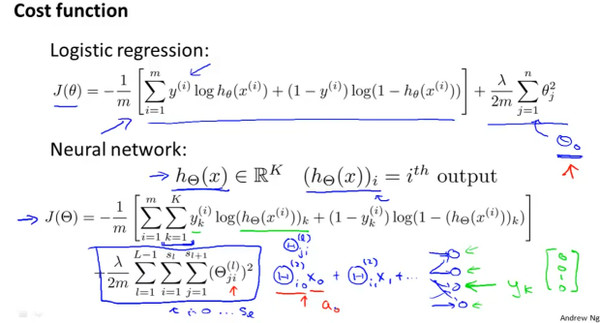
\includegraphics[width=0.6\textwidth]{Figuras/1520130384733.jpg}
\caption{Función de Costo}
\label{fig: Costo}
\end{figure}
\lipsum[1-9]

\begin{figure}[h]
	\centering
	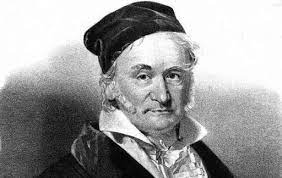
\includegraphics[width=0.6\textwidth]{Figuras/gauss.jpg}
	\caption{El Príncipe : Gauss}
	\label{fig : gauss}
\end{figure}
\lipsum[3]

\begin{figure}[h]
	\centering
	
\includegraphics[width=0.6\textwidth]{Figuras/JRR.jpg}
	\caption{Julio Ramon Ribeyro}
	\label{fig: Maestro}
\end{figure}

\lipsum[3-7]
\begin{figure}[h]
	\centering
	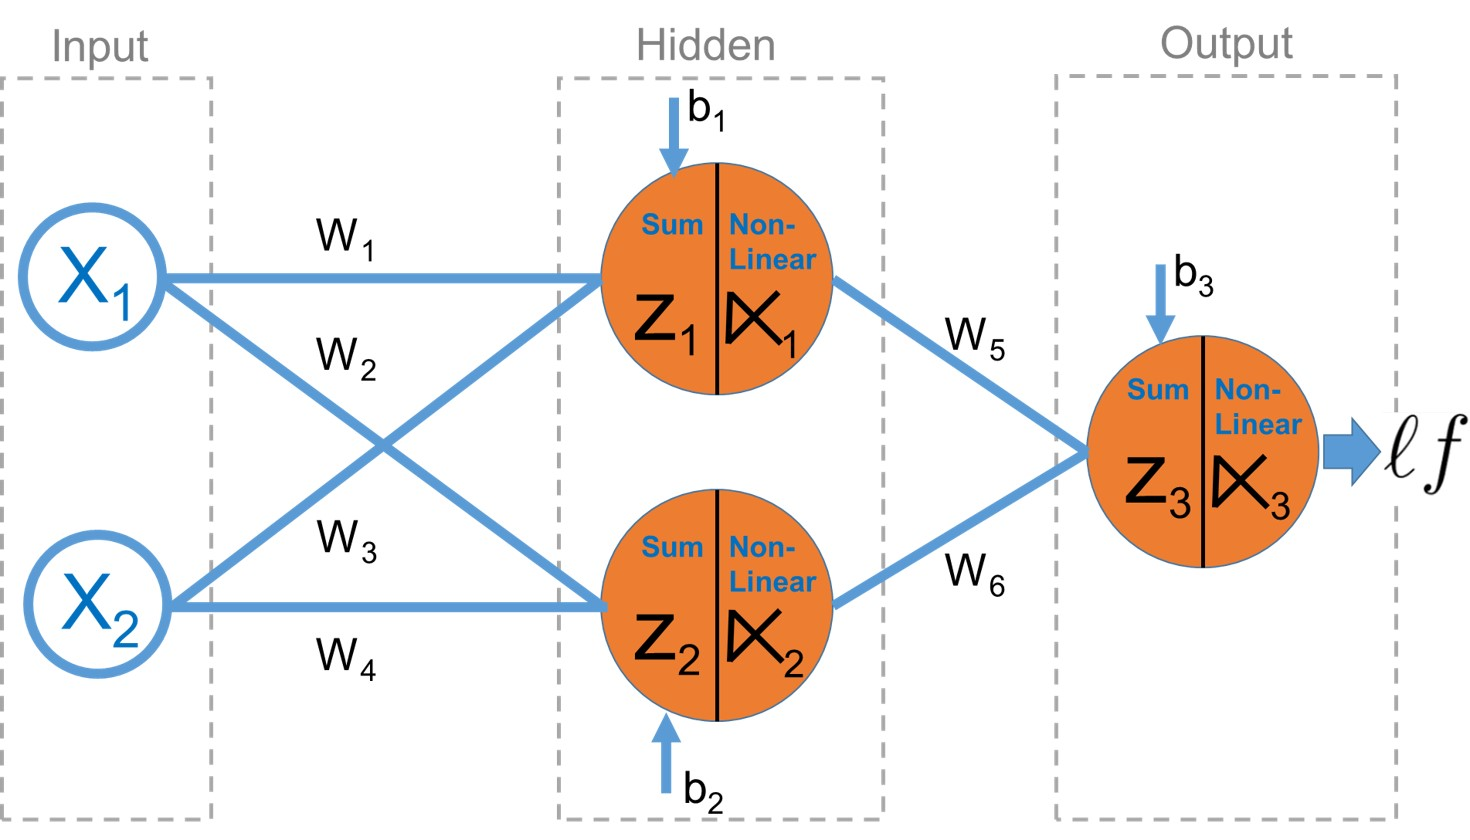
\includegraphics[width=0.6\textwidth]{Figuras/Maths-of-Deep-Learning-Neural-Networks-Image-3.jpg}
	\caption{Red Neuronal}
	\label{fig: perceptron}
\end{figure}


\section{Construcción del indice de tablas}
\lipsum[15]
\begin{table}[h]
	\centering
\begin{tabular}{cccr}
	\hline
	Producto & Precio Unitario & Cantidad & Subtotal \\
	\hline
	Monitores & 1250 & 2 & 2500\\
	& 2780 & 2 & 5560 \\
	& 16800 & 4 & 67200 \\
	\hline
	GPU	 	  & 2500 & 2 & 5000\\
	& 3700 & 3 & 11100\\
	\cline{4-4}
	&      &   & 78300
\end{tabular}
\caption{Costo de Monitor y Co-Procesador Matemático}
\label{table:1}
\end{table}

\lipsum[5-9]

\begin{table}[h]
	\centering
	\begin{tabular}{cccr}
		\hline
		Producto & Precio Unitario & Cantidad & Subtotal \\
		\hline
		Monitores & 1250 & 2 & 2500\\
		& 2780 & 2 & 5560 \\
		& 16800 & 4 & 67200 \\
		\hline
		GPU	 	  & 2500 & 2 & 5000\\
		& 3700 & 3 & 11100\\
		\cline{4-4}
		&      &   & 78300
	\end{tabular}
	\caption{Costo de Monitor y Co-Procesador Matemático - Versión 2}
	\label{table:2}
\end{table}

\lipsum[11-14]
\begin{table}[h]
	\centering
	\begin{tabular}{cccr}
		\hline
		Producto & Precio Unitario & Cantidad & Subtotal \\
		\hline
		Monitores & 1250 & 2 & 2500\\
		& 2780 & 2 & 5560 \\
		& 16800 & 4 & 67200 \\
		\hline
		GPU	 	  & 2500 & 2 & 5000\\
		& 3700 & 3 & 11100\\
		\cline{4-4}
		&      &   & 78300
	\end{tabular}
	\caption{Costo de Monitor y Co-Procesador Matemático - Tablita 3}
	\label{table:3}
\end{table}

FIN.
\newpage
\listoftables
\newpage
\listoffigures
\newpage
\tableofcontents
\end{document}

